\documentclass[xcolor=svgnames,t,final]{beamer}

\usepackage[T1]{fontenc}
\usepackage[utf8]{inputenc}
\usepackage{lmodern} % Smooth fonts : always use it

\usepackage[french]{babel}

%%%%%%% Page de titre %%%%%%%%%%

\title{Lois à densité \\ Corrigés des exemples du cours}\subtitle{Terminale S 734}
\author[]{Frédéric Junier \thanks{\url{http://frederic-junier.org/} }}
\institute[Lycée du Parc]{Lycée du Parc, Lyon}
\date[]{}

%%%%%%Environnements et symboles mathématiques%%%%

%%%Tableaux de variations %%%%%%%%%%

\usepackage{variations}

%%%%%%%%%%%AmsMaths%%%%%%
\usepackage{mathtools}        %Commandes essentielles, extension d'amsmath
\usepackage{amsfonts,amssymb}  %Principaux symboles
\usepackage{mathrsfs} %Polices calligraphiques
\usepackage{stmaryrd} %Pour les intervalles d'entiers avec \llbracket et \rrbracket
\usepackage[autolanguage, np]{numprint}
%%%%%%%%%%%%Là encore il y a de grosses différences entre le monde anglo-saxon et les francophones.Le séparateur des décimales est un point en anglais et une virgule en français. Leséparateur des milliers est une virgule en anglais et une espace insécable en français. Ilest préférable d’utiliser le package numprint (\usepackage{numprint}) qui associé àfrenchb produira la bonne typographie.
%123456789 = 123456789 \numprint{123456789} = 123 456 789  \numprint{3,1415926535897932384626} = 3,141 592 653 589 793 238 462 6  \numprint{12.34} = 12,34  En plus tu peux préciser les unités de cette façon : \numprint[kg]{12.34} = 12,34 kg ou encore \numprint[\degres C]{22} = 22°C Si tu veux utiliser le raccourci \np{} au lieu de \numprint{}, il te faut charger le package de cette façon : \usepackage[np]{numprint}

\usepackage{bbm, dsfont}   %Fonction indicatrice
\usepackage{esint,esvect}  %Flèches supplémentaires.

%%%%url%%%%

\usepackage{url}

%%%%%%%%%%%Packages spécifiques pour les sorties pdf%%%%%%%%

%%%%Insertion de liens hypertextes %%%%

\usepackage{hyperref}
            
            

%%%%%%%%%%%%Graphiques et Dessins%%%%%%%%%%%%%%

\usepackage{graphicx}		
%\rotatebox[origin=x0x1]{angle}{texte} avec xox1 parmi t (top) l (left) r (right) B (ligne de base) et b (bottomm)
%\resizebox{largeur}{hauteur}{texte} pour faire rentrer u nelement encombrant dans une boite	


%%%%%%%%%%Parametrages Beamer %%%%%%%%%%%%%%%%%

\usetheme{Singapore} % Beamer theme
\usecolortheme[named=Purple]{structure} % Color: latextemplates.com/svgnames-colors
\setbeamercolor{navigation symbols}{fg=black}
\setbeamertemplate{navigation symbols}{\insertframenumber}

%À mettre dans le préambule pour faire apparaitre le plan à chaque section 

\AtBeginSection
{
\begin{frame}
\frametitle{Plan}
\tableofcontents[current, currentsubsection]
\end{frame}
}
 

%%%%%%%%%%%%%%%%%%%%%%%%%%%%
%Le moteur eTeX est aujourd'hui utilisé par toutes les distributions (MikTeX, TeXlive) à la place de l'ancien TeX (en fait, c'est plutôt PDFTeX, le successeur de eTeX, qui est utilisé ; contrairement à ce que son nom indique, il peut produire du dvi). Le fait d'utiliser le moteur eTeX au lieu de TeX donne accès à des choses en plus (par exemple à \middle pour aller avec \left et \right, mais aussi à des commandes bien pratiques comme \numexpr, \dimexpr, \detokenize, etc. ainsi qu'à des ressources supplémentaires, comme plus de compteurs disponibles).

%Lorsqu'on utilise le moteur eTeX, certaines de ces fonctionnalités sont automatiquement accessibles (c'est le cas de \middle, \numexpr, etc.), mais pas d'autres (c'est le cas des compteurs supplémentaires). Pour activer ces fonctionnalités manquantes, on peut charger le package etex.sty. Ainsi, l'utilisation d'etex.sty est une solution courante au problème d'avoir trop de compteurs définis (c'est le cas si on charge ensemble trop de packages du type tikz, pstricks, xymatrix, ...)

%\usepackage{etex}

%%%%%%%%%%%%Graphiques%%%%%%%%%%%%%%
\usepackage{graphicx}	
%\rotatebox[origin=x0x1]{angle}{texte} avec xox1 parmi t (top) l (left) r (right) B (ligne de base) et b (bottomm)	
%\resizebox{largeur}{hauteur}{texte} pour faire rentrer u nelement encombrant dans une boite		
%\usepackage{pstricks,pst-plot,pst-text,pst-tree,pst-eps,pst-fill,pst-node,pst-math,pstricks-add,pst-xkey,pst-blur,pst-coil,pst-grad,pst-eucl}

%\begin{picture}(0,0) permet d'insérer n'importe quoi, n'importe où sans prendre de place (utilie pour annoter une figure en eps)
%Une autre technique est \makebox[0cm][alignement]{texte}
%Exemple:
%\includegraphics[scale=1]{singe.eps}
%\begin{picture}(0,0)
%\put(-27,10){$\sqrt[3]{8}$}
%\end{picture}
\usepackage{pgf,tikz}
\usetikzlibrary{arrows}
\usetikzlibrary{shapes.geometric}
\usetikzlibrary{petri}
\usetikzlibrary{decorations}
\usetikzlibrary{arrows}

%%%%%%%¨Puces%%%%%%%%%%%%
\usepackage{enumerate}


%%%%%%%%%%%%%%%%%%%%%%%%%%%%%%%%%%%%%%%%%%%%%%%%%%%%%%%%%%%%%%%%%%%%%%%%
%%%%%%%%%%%%%%%%%%%%Environnements persos%%%%%%%%%%%%%%%%%%%%%%%%%%%%%%%%
%Syntaxe :
%\newenvironment{nom}[nombre d'args][defaut]{definitions initiales}{definitions finales}
%definitions intiales sont les commandes appelées par \begin{nom}
%Definitions finales sont les commandes appelées par \end{nom}


%%%%%Package listings%%%%%%%%%%%%

\usepackage{listings}
%On utilise l?environnement lstlisting pour insérer
%un code source.
%En plus de l?environnement lstlisting, on peut également utiliser la
%commande \lstinline qui fonctionne comme la commande \verb, en ce
%sens qu?on peut utiliser n?importe quel caractère comme délimiteur. Enfin,
%la commande \lstinputlisting permet de charger un code source depuis
%un fichier externe.
%Il y a deux manières de préciser des options : soit via l?option de l?envi-
%ronnement ou de la commande, soit en utilisant la commande \lstset
%qui permet de définir des options de manière globale.

\lstset{ %
  language=Python,                % the language of the code
  basicstyle=\ttfamily,           % the size of the fonts that are used for the code
  numbers=left,                   % where to put the line-numbers
  numberstyle=\tiny,  % the style that is used for the line-numbers
  %stepnumber=2,                   % the step between two line-numbers. If it's 1, each line 
                                  % will be numbered
  %numbersep=5pt,                  % how far the line-numbers are from the code
  backgroundcolor=\color{white},      % choose the background color. You must add \usepackage{color}
  showspaces=false,               % show spaces adding particular underscores
  showstringspaces=false,         % underline spaces within strings
  showtabs=false,                 % show tabs within strings adding particular underscores
  %frame=single,                   % adds a frame around the code
  rulecolor=\color{black},        % if not set, the frame-color may be changed on line-breaks within not-black text (e.g. comments (green here))
  tabsize=4,                      % sets default tabsize to 2 spaces
  captionpos=b,                   % sets the caption-position to bottom
  breaklines=true,                % sets automatic line breaking
  breakatwhitespace=false,        % sets if automatic breaks should only happen at whitespace
  %title=\lstname,                   % show the filename of files included with \lstinputlisting;
                                  % also try caption instead of title
  breakindent=1cm,
  keywordstyle=\color{blue},          % keyword style
  commentstyle=\color{red},       % comment style
  %stringstyle=\ttfamily\color{green},         % string literal style
  escapeinside={\%*}{*)},            % if you want to add LaTeX within your code
  morekeywords={*,...},              % if you want to add more keywords to the set
  deletekeywords={...}              % if you want to delete keywords from the given language
  upquote=true,columns=flexible,
  frame=lines,
  extendedchars=true,
xleftmargin=1cm,xrightmargin=1cm
}


%\lstset{language=Python,basicstyle=\small , frame=single,tabsize=4,showspaces=false,showtabs=false,showstringspaces=false,numbers=left,numberstyle=\tiny , extendedchars=true}


%%%%%PAckages pour l'environnement algobox%%%%%%%%%%%%%%%%%%%%%%%%%%%%%%%%%%
\usepackage{algorithm}
\usepackage{algpseudocode}



%%%%%%%%%%%%%%%%%%Maths divers%%%%%%%%%%%%%%%%%%%%%%%%%
%Delimiteurs
\newcommand{\delim}[3]{\raise #1\hbox{$\left #2\vbox to #3{}\right.$}}


%%%%%%%%%%%%%Nombres%%%%%%%%%%%%%%%%

%Ensemble prive de...
%\newcommand{\prive}{\boi}%{\backslash}

%Ensembles de nombres%%%%%%%%%%%%%%%%%
\newcommand{\R}{\mathbb{R}}
\newcommand{\N}{\mathbb{N}}
\newcommand{\D}{\mathbb{D}}
\newcommand{\Z}{\mathbb{Z}}
\newcommand{\Q}{\mathbb{Q}}
\newcommand{\C}{\mathbb{C}}
\newcommand{\df}{~\ensuremath{]0;+\infty[}~}
\newcommand{\K}{\mathbb{K}}

%%%%%%%%Arithmetique%%%%%%%%%%
%PGCD, PPCM
\newcommand{\PGCD}{\mathop{\rm PGCD}\nolimits}
\newcommand{\PPCM}{\mathop{\rm PPCM}\nolimits}

%Intervalles
\newcommand{\interoo}[2]{]#1\, ;\, #2[}
\newcommand{\Interoo}[2]{\left]#1\, ;\, #2\right[}
\newcommand{\interof}[2]{]#1\, ;\, #2]}
\newcommand{\Interof}[2]{\left]#1\, ;\, #2\right]}
\newcommand{\interfo}[2]{[#1\, ;\, #2[}
\newcommand{\Interfo}[2]{\left[#1\, ;\, #2\right[}
\newcommand{\interff}[2]{[#1\, ;\, #2]}
\newcommand{\Interff}[2]{\left[#1\, ;\, #2\right]}
%\newcommand\interentiers #1#2{[\! [#1\, ;\, #2]\! ]}
\newcommand{\interentiers}[2]{\llbracket #1\, ;\, #2\rrbracket}
%


%%%%%%%%%%%%%%Nombres complexes%%%%%

\newcommand{\ic}{\text{i}}
%\newcommand{\I}{\text{i}}
\newcommand{\im}[1]{\text{Im}\left(#1\right)}
\newcommand{\re}[1]{\text{Re}\left(#1\right)}
\newcommand{\Arg}[1]{\text{arg}\left(#1\right)}
\newcommand{\Mod}[1]{\left[#1\right]}
%Parties entière, réelle, imaginaire, nombre i
\newcommand{\ent}[1]{\text{E}\left(#1\right)}
\renewcommand{\Re}{\mathop{\rm Re}\nolimits}
\renewcommand{\Im}{\mathop{\rm Im}\nolimits}
\renewcommand{\i}{\textrm{i}}

%%%%%%%%%%%Probabilites et statistiques%%%%%
\newcommand{\loibinom}[2]{\mathcal{B}\left(#1\ ; \ #2 \right)}
\newcommand{\loinorm}[2]{\mathcal{N}\left(#1\ ; \ #2 \right)}
\newcommand{\loiexp}[1]{\mathcal{E}\left(#1\right)}
\newcommand{\proba}[1]{\text{P}\big(#1\big)}
\newcommand{\probacond}[2]{\text{P}_{#2}\big(#1\big)}
\newcommand{\esperance}[1]{\text{E}\left(#1\right)}
\newcommand{\variance}[1]{\text{V}\left(#1\right)}
\newcommand{\ecart}[1]{\sigma\left(#1\right)}
\newcommand{\dnormx}{\frac{1}{\sqrt{2\pi}} \text{e}^{-\frac{x^2}{2}}}
\newcommand{\dnormt}{\frac{1}{\sqrt{2\pi}} \text{e}^{-\frac{t^2}{2}}}
\newcommand{\nbalea}[2]{\reinitrand[first=#1, last=#2, counter=num]  \rand $\thenum$}  %retourne un entier aleatoire antre les bornes #1 et #2 comprises
%Covariance
\newcommand{\cov}{\mathop{\rm cov}\nolimits}
%


%%%%%%%%%%Analyse%%%%%%%%%%%

%%%%%%%%%%%Courbe%%%%%%%%%%%%
\newcommand{\courbe}[1]{\ensuremath{\mathcal{C}_{#1}}}

%%%%%%%Fonction exponentielle%%%%%
\newcommand{\fe}{~fonction exponentielle~}
\newcommand{\e}{\text{e}}

%Fonction cotangente
\newcommand{\cotan}{\mathop{\rm cotan}\nolimits}
%%%%%%%%%%%%%%%%%%%%%%%%%%%%%%%%%%%%%%%%%
%
%Fonctions hyperboliques
\newcommand{\ch}{\mathop{\rm ch}\nolimits}
\newcommand{\sh}{\mathop{\rm sh}\nolimits}


%%%%%%%%%%%%%%Limites%%%%%%
\newcommand{\limite}[2]{\lim\limits
_{x \to #1} #2}
\newcommand{\limitesuite}[1]{\lim\limits
_{n \to +\infty} #1}
\newcommand{\limiteg}[2]{\lim\limits
_{\substack{x \to #1 \\ x < #1 }} #2}
\newcommand{\limited}[2]{\lim\limits
_{\substack{x \to #1 \\ x > #1 }} #2}

%%%%%%%%%%Continuité%%%%%%%%%%%
\newcommand{\TVI}{théorème des valeurs intermédiaires}

%%%%%%%%%%%Suites%%%%%%%%%%%%
\newcommand{\suite}[1]{\ensuremath{\left(#1_{n}\right)}}
\newcommand{\Suite}[2]{\ensuremath{\left(#1\right)_{#2}}}
%

%%%%%%%%%%%%%%%Calcul intégral%%%%%%
\newcommand{\dx}{\ensuremath{\text{d}x}}		% dx
\newcommand{\dt}{\ensuremath{\text{d}t}}		% dt
\newcommand{\dtheta}{\ensuremath{\text{d}\theta}}		% dtheta
\newcommand{\dy}{\ensuremath{\text{d}y}}		% dy
\newcommand{\dq}{\ensuremath{\text{d}q}}		% dq

%%%Intégrale%%%
\newcommand{\integralex}[3]{\int_{#1}^{#2} #3 \ \dx}
\newcommand{\integralet}[3]{\int_{#1}^{#2} #3 \ \dt}
\newcommand{\integraletheta}[3]{\int_{#1}^{#2} #3 \ \dtheta}

%%%%%Equivalent%%
\newcommand{\equivalent}[1]{\build\sim_{#1}^{}}

%o et O%%%%
\renewcommand{\o}[2]{\build o_{#1\to #2}^{}}
\renewcommand{\O}[2]{\build O_{#1\to #2}^{}}



%%%%%%%%%%%%%%%Geometrie%%%%%%%%%%%%%%%%%%%%%%%

%%%%%%%%%%%%%%%Reperes%%%%%%%%%%%%%%
\def\Oij{\ensuremath{\left(\text{O},~\vect{\imath},~\vect{\jmath}\right)}}
\def\Oijk{\ensuremath{\left(\text{O},~\vect{\imath},~ \vect{\jmath},~ \vect{k}\right)}}
\def\Ouv{\ensuremath{\left(\text{O},~\vect{u},~\vect{v}\right)}}
\renewcommand{\ij}{(\vec\imath\, ;\vec\jmath\,)}
\newcommand{\ijk}{(\vec\imath\, ;\vec\jmath\, ;\vec k\,)}
\newcommand{\OIJ}{(O\,;\, I\,;\, J\,)}
\newcommand{\repere}[3]{\big(#1\, ;\,\vect{#2} ;\vect{#3}\big)}
\newcommand{\reperesp}[4]{\big(#1\, ;\,\vect{#2} ;\vect{#3} ;\vect{#4}\big)}

%%%%%%%%%Coordonnees%%%%%%%%%%%%%%
\newcommand{\coord}[2]{(#1\, ;\, #2)}
\newcommand{\bigcoord}[2]{\big(#1\, ;\, #2\big)}
\newcommand{\Coord}[2]{\left(#1\, ;\, #2\right)}
\newcommand{\coordesp}[3]{(#1\, ;\, #2\, ;\, #3)}
\newcommand{\bigcoordesp}[3]{\big(#1\, ;\, #2\, ;\, #3\big)}
\newcommand{\Coordesp}[3]{\left(#1\, ;\, #2\, ;\, #3\right)}

%Symboles entre droites
%\newcommand{\paral}{\sslash}
\newcommand{\paral}{\mathop{/\!\! /}}
%
%%%%%%%%%Produit scalaire, Angles%%%%%%%%%%
\newcommand{\scal}[2]{\vect{#1} \, \cdot \, \vect{#2}}
\newcommand{\Angle}[2]{\left(\vect{#1} \, , \, \vect{#2}\right)}
\newcommand{\Anglegeo}[2]{\left(\widehat{\vect{#1} \, , \, \vect{#2}}\right)}
\renewcommand{\angle}[1]{\widehat{#1}}
\newcommand{\anglevec}[2]{\left(\vec {#1}\, ,\,\vec {#2} \right)}
\newcommand{\anglevecteur}[2]{(#1\, ,\, #2)}
\newcommand{\Anglevec}[2]{(\vecteur{#1}\, ,\,\vecteur{#2})}
\newcommand{\prodscal}[2]{#1 \, \cdot \, #2}

%Arc
%\newcommand{\arc}[1]{\wideparen{#1}}
\newcommand{\arcoriente}[1]{\overset{\curvearrowright}{#1}}
%
%


%%%%%%%%%%%%%%%Normes%%%%%%%%%%%%%%%%
\newcommand{\norme}[1]{\left\| #1\right\|}
\newcommand{\normebis}[1]{\delim{2pt}{\|}{9pt}\! #1\delim{2pt}{\|}{9pt}}
\newcommand{\normetriple}[1]{\left |\kern -.07em\left\| #1\right |\kern -.07em\right\|}
\newcommand{\valabs}[1]{\big| \, #1 \, \big|}
%

%%%%%%%%%%%%%%%%%%%%%%%%%%%Degré%%%%%%
%\newcommand{\Degre}{\ensuremath{^\circ}}
%La commande \degre est déjà définie dans le package babel

%%%%%%%%%%Vecteurs%%%%%%%%%%%
\newcommand{\vect}[1]{\mathchoice%
{\overrightarrow{\displaystyle\mathstrut#1\,\,}}%
{\overrightarrow{\textstyle\mathstrut#1\,\,}}%
{\overrightarrow{\scriptstyle\mathstrut#1\,\,}}%
{\overrightarrow{\scriptscriptstyle\mathstrut#1\,\,}}}



%%%%%%%%%%%%%Algebre%%%%%%%%%%%%%%%


%%%%%%%%%%Systemes%%%%%%%%%%%
%Systemes
\newcommand{\sys}[2]{
\left\lbrace
 \begin{array}{l}
  \negthickspace\negthickspace #1\\
  \negthickspace\negthickspace #2\\
 \end{array}
\right.\negthickspace\negthickspace}
\newcommand{\Sys}[3]{
\left\lbrace
 \begin{array}{l}
  #1\\
  #2\\
  #3\\
 \end{array}
\right.}
\newcommand{\Sysq}[4]{
\left\lbrace
 \begin{array}{l}
  #1\\
  #2\\
  #3\\
  #4\\
 \end{array}
\right.}
%
%

%%%%%%%%%%%%%%%%Matrices%%%%%%%%%%%%%%%%%%
%Comatrice
\newcommand{\com}{\mathop{\rm com}\nolimits}
%
%
%Trace
\newcommand{\tr}{\mathop{\rm tr}\nolimits}
%
%
%Transposee
\newcommand{\transposee}[1]{{\vphantom{#1}}^t\negmedspace #1}
%
%
%Noyau
\newcommand{\Ker}{\mathop{\rm Ker}\nolimits}
%
%

%
%Matrices
\newcommand{\Mn}{\mathcal M_n}
\newcommand{\matrice}[4]{
\left(
 \begin{array}{cc}
  #1 & #2 \\
  #3 & #4
 \end{array}
\right)}

\newcommand{\Matrice}[9]{
\left(
 \begin{array}{ccc}
  #1 & #2 & #3\\
  #4 & #5 & #6\\
  #7 & #8 & #9
 \end{array}
\right)}
\newcommand{\Vect}[3]{
\left(\negmedspace
 \begin{array}{c}
  #1\\
  #2\\
  #3
 \end{array}\negmedspace
\right)}
\newcommand{\Ideux}{\matrice{1}{0}{0}{1}}
\newcommand{\Itrois}{\Matrice{1}{0}{0}{0}{1}{0}{0}{0}{1}}
%
%
%Determinants
\newcommand{\determinant}[4]{
\left|
 \begin{array}{cc}
  #1 & #2 \\
  #3 & #4
 \end{array}
\right|}
\newcommand{\Determinant}[9]{
\left|
 \begin{array}{ccc}
  #1 & #2 & #3\\
  #4 & #5 & #6\\
  #7 & #8 & #9
 \end{array}
\right|}



%%%%%%%%%%%%%%%%%%%%%%%%%%%%%%%%%%%%%%%
%%%%%%%%%%%Commandes Tikz%%%%%%%%%%%%%%%

% Définition des nouvelles options xmin, xmax, ymin, ymax
% Valeurs par défaut : -3, 3, -3, 3
\tikzset{
xmin/.store in=\xmin, xmin/.default=-3, xmin=-3,
xmax/.store in=\xmax, xmax/.default=3, xmax=3,
ymin/.store in=\ymin, ymin/.default=-3, ymin=-3,
ymax/.store in=\ymax, ymax/.default=3, ymax=3,
}
% Commande qui trace la grille entre (xmin,ymin) et (xmax,ymax)
\newcommand {\grille}[1]
{\draw[help lines] (\xmin,\ymin) grid[step=#1] (\xmax,\ymax);}
% Commande \axes
\newcommand {\axes} {
\draw[->,very thick] (\xmin,0) -- (\xmax,0);
\draw[->,very thick] (0,\ymin) -- (0,\ymax);
\draw (\xmax, 0) node[above] {$x$};
\draw (0, \ymax) node[left] {$y$};
}
% Commande qui limite l?affichage à (xmin,ymin) et (xmax,ymax)
\newcommand {\fenetre}
{\clip (\xmin,\ymin) rectangle (\xmax,\ymax);}

%Exemple d'utilisation

%\begin{center}
%\begin{tikzpicture} [xmin=-2,xmax=2,ymin=0,ymax=5]
%\grille{1} \axes \fenetre
%\draw plot[smooth] (\x,\x^2);
%\end{tikzpicture}
%\end{center}


%%%%%%%%%%%%%%%%%%%%%%%%%%%%%%%%%%%%%%%%
%%%%%%%%%%%Fin Commandes Tikz%%%%%%%%%%%%%%%


%%%%%%Cadre Maxima%%%%%%%
\definecolor{labelcolor}{RGB}{100,0,0}


%%%%%%%Symbole pour code calculatrice%%%%%%

%Flèche remplie pour défilement de menu

\newcommand{\flechefillright}{
\begin{tikzpicture}[scale=0.15] \fill (0,0)--(2,1)--(0,2)--cycle;
\end{tikzpicture}}

%%%%%%%%%%%%%Symboles pour calculatrice Casio%%%%
\newcommand{\execasio}{\Pisymbol{psy}{191}} %Retour chariot
\newcommand{\dispcasio}{\begin{pspicture}(.1,.1)\pspolygon*(.1,0)(.1,.1)\end{pspicture}} %Triangle « Disp »
\newcommand{\dispcasiotikz}{\begin{tikzpicture}[scale=0.2]
\fill (0,0) -- (1,0) -- (1,1) -- cycle;
\end{tikzpicture}} %Triangle « Disp »
%
%
%Fleche entre deux lignes, d'apres 'un bon petit' : http://forum.mathematex.net/latex-f6/fleches-entre-deux-lignes-pour-resolution-d-equation-t10283.html#p99817
\newcommand\addnode[1]{\Rnode{#1}{}}
\newcommand\linknode[3]{\ncbar[angleA=0,angleB=0,nodesep=1ex,arm=10ex,offset=-2pt]{->}{#1}{#2}\Aput{\vphantom{x}#3}}

%%%%%Fin des commandes Mathematiques%%%%%%%%

\everymath{\displaystyle}

\begin{document}

\frame{\titlepage}


\begin{frame}
\frametitle{Table des matières}
\begin{itemize}
	\item \hyperlink{exemple1}{Exemple 1}
	\item \hyperlink{exemple2}{Exemple 2}
	\item \hyperlink{exemple3}{Exemple 3}
	\item \hyperlink{exemple4}{Exemple 4}
	\item \hyperlink{exemple5}{Exemple 5}
	\item \hyperlink{exemple6}{Exemple 6}
		\item \hyperlink{exemple7}{Exemple 7}
			\item \hyperlink{exemple8}{Exemple 8}
			\item \hyperlink{exemple9}{Exemple 9}
				\item \hyperlink{exemple10}{Exemple 10}
						\item \hyperlink{exemple11}{Exemple 11}
						\item \hyperlink{exemple12}{Exemple 12}
						\item \hyperlink{exemple13}{Exemple 13}
						\item \hyperlink{exemple14}{Exemple 14}
\end{itemize}

\end{frame}



\begin{frame}

\frametitle{Exemple 1 : Partie 1}

\label{exemple1}
Sofia utilise le bus pour se rendre au cinéma.  La durée du trajet entre son domicile et le cinéma (exprimée en minutes) est une variable aléatoire $T$ qui prend des valeurs choisies aléatoirement dans l'intervalle $[12~;~15]$. On dit que $T$ suit la loi uniforme sur l'intervalle $[12~;~15]$. La probabilité que la durée de trajet appartienne à un intervalle $\Interff{a}{b}$ inclus dans $[12~;~15]$ est alors proportionnelle à la longueur de cet intervalle.

\begin{itemize}
\item L'événement $\left\{12 \leqslant  T \leqslant 15\right\}$ est égal à l'univers $\Omega$ de cette expérience aléatoire, donc   $\proba{12 \leqslant T \leqslant 15}=1$.
	\item La probabilité de l'événement A = \og{} \textit{la durée du trajet de Sofia est  inférieure ou égale à $13$ minutes} \fg{} est proportionnelle à la longueur de l'intervalle $\Interff{12}{13}$, égale à $1$. Sachant que $\proba{12 \leqslant T \leqslant 15}=1$ et que la longueur de $\Interff{12}{15}$ est $3$, on a :	
\begin{equation*}
\proba{A}=\proba{12 \leqslant T \leqslant 13}=\frac{13-12}{15-12}=\frac{1}{3}
\end{equation*}


\end{itemize}


\end{frame}


\begin{frame}

\frametitle{Exemple 1 : Partie 2}




\begin{itemize}


	\pause \item De même la probabilité de l'événement B = \og{} \textit{la durée du trajet de Sofia est strictement supérieure à $13$ minutes} \fg{} est égale à :
\begin{equation*}
\proba{B}=\proba{13 <T \leqslant 15}=\frac{15 - 13}{15-12}=\frac{2}{3}
\end{equation*}
	
	\pause	\item L'événement C = \og{} \textit{la durée du trajet de Sofia est égale exactement à $13$ minutes} \fg{} est tel que  les événements A, B et C sont deux à deux incompatibles et $A \cup B \cup C= \Omega$. Les événements A, B et C forment une partition de l'univers donc $\proba{A}+\proba{B}+\proba{C}=1$.
		
Or on a $\proba{A}+\proba{B}=\frac{1}{3}+\frac{2}{3}=1$ donc $\proba{C}=0$.

On peut aussi calculer comme précédemment par proportionnalité : $\proba{C}=\proba{13 \leqslant T \leqslant 13}=0$

Comme il existe une infini d'instants dans l'intervalle $\Interff{12}{15}$ il n'est pas possible d'avoir la probabilité d'un instant non nulle et $\proba{12\leqslant T \leqslant 15}=1$.

		


\end{itemize}



\end{frame}


\begin{frame}

\frametitle{Exemple 1 : Partie 3}



\begin{itemize}

\item Une variable aléatoire $X$ donnant la face du dessus lorsqu'on lance un dé à six faces équilibré suit une \textbf{loi uniforme discrète} à valeurs dans l'ensemble $X(\Omega)=\{1;2;3;4;5;6\}$. On dit que $T$ suit une \textbf{loi uniforme continue} à valeurs dans l'intervalle $[12~;~15]$. 
La différence principale entre une loi discrète et une loi continue est le nombre d'éléments (le cardinal) de l'univers : infini pour une loi continue et fini  pour une loi discrète.

		
\end{itemize}



\end{frame}




\begin{frame}

\frametitle{Exemple 1 : Partie 4}



\begin{itemize}


		\item Représenter dans un repère du plan la courbe de la fonction $f$ définie sur l'intervalle $[12~;~15]$ par $f(t)=\frac{1}{3}$ puis hachurer des domaines d'aires égales à $\proba{\text{A}}$ et $\proba{\text{B}}$.
		
		
		\begin{center}
		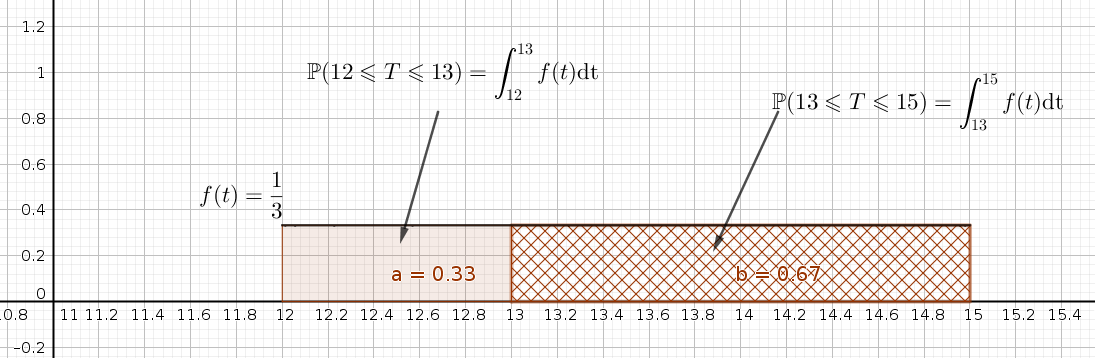
\includegraphics[scale=0.25]{images/exemple1.png}
		\end{center}
		
		
\end{itemize}



\end{frame}


\begin{frame}

\frametitle{Exemple 1 : Partie 5}



\begin{itemize}


		\item Pour  estimer la durée moyenne du trajet de Sofia, on peut s'inspirer de la formule de l'espérance de la variable aléatoire discrète $X$ :  $\esperance{X}=\sum_{k=1}^{6}k \proba{X=k}$. Comparaison entre la variable aléatoire $X$ suivant une loi discrète uniforme et la loi $T$ qui suit une loi uniforme continue :
\pause	 \item 		\begin{center}
	\begin{tabular}{|c|c|c|}
		\hline 
		 & loi discrète X & loi continue T \\ 
		\hline 
		valeur & $k \in \{1,2,3,4,5,6\}$ & $t \in \Interff{12}{15}$ \\ 
		\hline 
		probabilité & $\proba{X=k}$ &  $\int_{a}^{b}f(t)\text{dt}$ \\ 
		\hline 
		espérance & $\sum_{k=1}^{6}k \proba{X=k}$ & $\int_{12}^{15}tf(t)\text{dt}$ \\ 
		\hline 
		\end{tabular} 	
		\end{center}
	
		

\end{itemize}



\end{frame}



\begin{frame}

\frametitle{Exemple 1 : Partie 6}






L'espérance de $T$, durée moyenne du trajet de Sofia, peut être estimée ainsi : 

\pause			\begin{equation*}
\int_{12}^{15}tf(t)\text{dt}=\int_{12}^{15}\frac{t}{3}\text{dt}=\frac{1}{3}\left[\frac{t^{2}}{2 \times (15-12)}\right]_{12}^{15}=\frac{15+12}{2} = 13,5 
		\end{equation*}
On trouver le centre de l'intervalle $\Interff{12}{15}$ ce qui et conforme à l'intuition.



\end{frame}

\begin{frame}

\frametitle{Exemple 2 : Partie 1}

Vérifions que $f: t \mapsto \frac{1}{5}$ est une densité de probabilité sur $I=\Interff{2}{7}$.

\begin{itemize}
\pause \item \textbf{point 1 :} $f$ est continue sur $I=\Interff{2}{7}$.



\pause \item \textbf{point 2 :} $f$ est à valeurs positives.

\pause \item \textbf{point 3 :} $\int_{2}^{7}\frac{1}{5}\text{dt} = \left[\frac{t}{5}  \right]_{2}^{7}=\frac{7-2}{5}=1$

\end{itemize}

$f$ est donc bien une fonction de densité de probabilité.


\end{frame}

\begin{frame}

\frametitle{Exemple 2 : Partie 1}

 Soit $F$ la fonction définie sur $\R^{+}$ par $F(t)=1-(2t+1)\text{e}^{-2t}$.
 
\begin{itemize}
\pause \item $F$ est dérivable sur $\R^{+}$ par règles opératoire et pour tout réel $t \geqslant 0$, on a :
\begin{equation*}
F'(t)=0-2\text{e}^{-2t}+2(2t+1)\text{e}^{-2t}=4t\text{e}^{-2t}=f(t)
\end{equation*}

\pause \item La fonction  $f$ définie sur $\Interfo{0}{+\infty}$ par $f(t)=4t\text{e}^{-2t}$ est dérivable donc continue sur $\Interfo{0}{+\infty}$ et  elle est positive sur cet intervalle. 

De plus pour tout réel $x\geqslant 0$, on a $\integralet{0}{x}{f(t)}=F(x)-F(0)= 1-(2x+1)\text{e}^{-2x}$ et $\limite{+\infty}{F(x)}=1$ par composition et somme. On a donc bien $\lim\limits_{x\to +\infty}\integralet{0}{x}{f(t)}=1$.

$f$ est donc  une fonction de densité de probabilité sur $\R^{+}$.
\pause \item Soit $X$ une variable aléatoire de densité $f$, on a :
$$P\left(2<X<3\right)=\int_{2}^{3}f(t)\text{dt}=F(3)-F(2)=5\text{e}^{-4}-7\text{e}^{-6}$$
\end{itemize}


\end{frame}


\begin{frame}

\frametitle{Exemple 2 : Partie 1}

 Soit $F$ la fonction définie sur $\R^{+}$ par $F(t)=1-(2t+1)\text{e}^{-2t}$.
 
\begin{itemize}
\item La fonction  $f$ définie sur $\Interfo{0}{+\infty}$ par $f(t)=4t\text{e}^{-2t}$ est dérivable donc continue sur $\Interfo{0}{+\infty}$ et  elle est positive sur cet intervalle. 

De plus pour tout réel $x\geqslant 0$, on a $\integralet{0}{x}{f(t)}=F(x)-F(0)= 1-(2x+1)\text{e}^{-2x}$ et $\limite{+\infty}{F(x)}=1$ par composition et somme. On a donc bien $\lim\limits_{x\to +\infty}\integralet{0}{x}{f(t)}=1$.

$f$ est donc  une fonction de densité de probabilité sur $\R^{+}$.
\pause \item Soit $X$ une variable aléatoire de densité $f$, on a :
$$P\left(2<X<3\right)=\int_{2}^{3}f(t)\text{dt}=F(3)-F(2)=5\text{e}^{-4}-7\text{e}^{-6}$$
\end{itemize}


\end{frame}



\begin{frame}

\frametitle{Exemple 3: Partie 1}
\label{exemple3}


Soit $X$ une variable aléatoire de densité $f(t)=3\,\text{e}^{ -3t} $ sur $\R^{+}$.

On recherche deux  réels $a, b$ tels que $G: t \mapsto (at+b)\text{e}^{-3t}$ soit une primitive de la fonction $ t \mapsto tf(t)$.


\begin{itemize}
\pause \item $G$ est dérivable sur $\R_{+}$ et pour tout réel $t \geqslant 0$, on a :
$$G'(t)=a\text{e}^{-3t}-3(at+b)\text{e}^{-3t}$$
On a donc $G'(0)=a-3b$ et $G'(1)=\text{e}^{-3}(-2a-3b)$.
Si pour tout $t \geqslant 0$, on a  $G'(t)=tf(t)$ alors :

$$\begin{cases}G'(0)=0 \\ G'(1)=f(1)\end{cases}\Leftrightarrow \begin{cases}a-3b=0 \\\text{e}^{-3}(-2a-3b)=3\text{e}^{-3}\end{cases}\Leftrightarrow \begin{cases}b =-\frac{1}{3} \\  a =-1 \end{cases}$$

Réciproquement, on peut vérifier que la fonction $G$ définie sur $\R_{+}$  par $G(t)=(-t-\frac{1}{3})\text{e}^{-3t}$ a pour fonction dérivée $tf(t)$.

\end{itemize}

\end{frame}




\begin{frame}

\frametitle{Exemple 3: Partie 2}
\label{exemple3}


Soit $X$ une variable aléatoire de densité $f(t)=3\,\text{e}^{ -3t} $ sur $\R^{+}$.

On recherche deux  réels $a, b$ tels que $G: t \mapsto (at+b)\text{e}^{-3t}$ soit une primitive de la fonction $ t \mapsto tf(t)$.


\begin{itemize}

\pause \item Pour déterminer l'espérance de la variable aléatoire $X$, on fixe d'abord $x \geqslant 0$ et on calcule $\int_{0}^{x}tf(t)\text{dt}=\left[G(t)\right]_{0}^{x}=G(x)-G(0)=(-x-\frac{1}{3})\text{e}^{-3x} + \frac{1}{3}$.
Par composition (avec règle de croissances comparées $\limite{+\infty}{\frac{x}{\text{e}^{x}}}=0$) et somme on a $\limite{+\infty}{G(x)}=0$, donc par somme on a $\limite{+\infty}{\int_{0}^{x}tf(t)\text{dt}}=\frac{1}{3}$.

L'espérance de la variable aléatoire $X$ est donc $\frac{1}{3}$.
\end{itemize}

\end{frame}







\begin{frame}

\frametitle{Exemple 4 : Partie 1}
\label{exemple4}

Un détaillant constate que ses melons se vendent bien lorsque leur masse est comprise entre $900$ g et
\np{1200}~g. Dans la suite, de tels melons sont qualifiés \og conformes \fg.

Le détaillant achète ses melons auprès d'un   maraîcher chez lequel, la masse en gramme  des melons est
 modélisée par une variable aléatoire $M$
qui suit une loi uniforme sur l'intervalle $[850~;~x]$, où $x$ est un nombre réel supérieur à \np{1200}.


\begin{itemize}

\pause \item Le détaillant constate que 75\,\% des melons du maraîcher sont conformes. %Déterminer $x$.

Autrement dit, la probabilité qu'un melon du maraîcher soit conforme est $0,75$; on a donc $P\left ( M} \in \cd 900~,~\np{1200}\cg \right ) = 0,75$.

Comme la variable aléatoire $M$ suit une loi uniforme sur $[ 850~,~x ]$, on a\\
$P\left ( M \in [ 900~,~\np{1200}]  \right ) = \dfrac{\np{1200}-900}{x-850}$.

On en déduit que $\dfrac{\np{1200}-900}{x-850} = 0,75$ ce qui équivaut à
$300 = 0,75x - 637,5$ ou à $937,5 = 0,75x$ c'est-à-dire $x=\np{1250}$.

\end{itemize}

\end{frame}



\begin{frame}

\frametitle{Exemple 4 : Partie 2}


Calcul de la masse moyenne d'un melon.

\begin{itemize}

\pause \item La masse d'un melon produit par le maraîcher suit une loi uniforme sur l'intervalle $[850;1250]$ donc   la masse moyenne d'un melon sur un échantillon de grande taille peut être approchée par l'espérance de $M$ égale à $\frac{850+1250}{2}=1050$ grammes.

\end{itemize}



\end{frame}

\begin{frame}

\frametitle{Exemple 5 : Partie 1}

On note $X$ la variable aléatoire qui donne le nombre de kilomètres parcourus par un pneu, sans crevaison. On fait l'hypothèse que X suit une loi exponentielle de paramètre $\lambda$.

Montrer que $P(500\leqslant X\leqslant 1000) =\mathrm{e}^{-500\lambda}-\mathrm{e}^{\nombre{1000}\lambda}$.

\begin{itemize}

\pause \item 
On a $p(500 \leqslant X \leqslant 1000) = \displaystyle\int_{0}^{1000}\lambda\mathrm{e}^{-\lambda x}\:\text{d}x - \displaystyle\int_{0}^{500}\lambda\mathrm{e}^{-\lambda x}\:\text{d}x = \displaystyle\int_{500}^{1000}\lambda\mathrm{e}^{-\lambda x}\:\text{d}x = \left[\text{e}^{-\lambda x} \right]_{500}^{1000} = - \text{e}^{-1000\lambda} - \left(\text{e}^{-500\lambda} \right) = \text{e}^{-500\lambda} - \text{e}^{-1000\lambda}$.

\end{itemize}



\end{frame}


\begin{frame}

\frametitle{Exemple 5 : Partie 2}

La probabilité que le pneu parcoure entre 500 et \nombre{1000} kilomètres sans crevaison étant égale à $\dfrac{1}{4}$, déterminer la valeur de $\lambda$.

\begin{itemize}

\pause \item 
On a donc $p(500 \leqslant X \leqslant 1000) = \dfrac{1}{4} \iff \text{e}^{-500\lambda} - \text{e}^{-1000\lambda} = \dfrac{1}{4} \iff \text{e}^{-500\lambda} - \left(\text{e}^{-500\lambda} \right)^2 - \dfrac{1}{4} = 0$.
En posant $x = \text{e}^{-500\lambda}$, l'équation à résoudre s'écrit 

$x - x^2 - \dfrac{1}{4} = 0 \iff x^2 - x + \dfrac{1}{4} = 0 \iff \left(x - \dfrac{1}{2} \right)^2  = 0 \iff x - \dfrac{1}{2} = 0 \iff x = \dfrac{1}{2}$.
Il reste à résoudre :
$\text{e}^{-500\lambda} = \dfrac{1}{2}$ soit d'après la croissance de la fonction $\ln,\: -500\lambda = \ln \left(\dfrac{1}{2}\right) \iff $

$-500\lambda = - \ln 2 \iff \lambda = \dfrac{\ln 2}{500}\approx \nombre{0,00138} \approx \nombre{0,0014}$.

\end{itemize}



\end{frame}


\begin{frame}


\frametitle{Exemple 6 Question 1}
\label{exemple6}


La durée de vie, en années, d'un composant électronique fabriqué dans une usine, est une variable aléatoire $T$ qui suit une loi exponentielle de paramètre $\lambda$ (où $\lambda$ est un nombre réel strictement positif).

Démontrer que $\lim\limits_{t \to + \infty} \proba{T \leqslant t}=1$.

\begin{itemize}
\item Soit $t\in[0,+\infty[$ :

$\begin{array}[t]{lcl}
\text{P}(T\leqslant t)&=&\int\limits_{0}^{t}f(x)\text{d}x=\int\limits_{0}^{t}\lambda \text{e}^{-\lambda x}\text{d}x\\
&=&\left[ -\text{e}^{-\lambda x}\right]_{0}^{t}=\left( -\text{e}^{-\lambda t}\right)-\left( -\text{e}^{-\lambda \times 0}\right\\ 
&=&\left( -\text{e}^{-\lambda t}\right)-(-1) =1-\text{e}^{-\lambda t}   
\end{array}$		
\[ \forall t\in[0,+\infty[\quad \text{P}(T\leqslant t)=1-\text{e}^{-\lambda t}\]

\end{itemize}


\end{frame}


\begin{frame}


\frametitle{Exemple 6 Question 1}


\begin{itemize}
\pause \item Soit $t\in[0,+\infty[$ :

De $\sys{l}{\lim\limits_{t\to +\infty}-\lambda t\overset{\red \lambda >0}{=}-\infty\\ \text{et}\\ \lim\limits_{X\to -\infty}\text{e}^X=0}$on déduit, par composition : 
$\lim\limits_{t\to +\infty}\text{e}^{-\lambda t}=0$.

On a ensuite, par somme : $\lim\limits_{t\to +\infty}(1-\text{e}^{-\lambda t})=1-0=1$ :	
\[\red \lim\limits_{t\to +\infty}\text{P}(T\leqslant t)=1\]	

\end{itemize}


\end{frame}



\begin{frame}


\frametitle{Exemple 6 Question 2)}
On suppose que $\proba{T \leqslant 7}=0,5$. Déterminer $\lambda$ à $10^{-3}$ près.

\begin{itemize}
\pause \item L'hypothèse s'écrit : $1-\text{e}^{-7\lambda}=0,5\quad (1)$

$\begin{array}[t]{lcl}
(1)&\iff&\text{e}^{-7\lambda}=0,5\\
&&\\
&\iff&-7\lambda=\ln \dfrac{1}{2} \\
&&\\
&\iff&-7\lambda=-\ln 2 \\
&&\\
&\iff&\lambda=\dfrac{\ln 2}{7}
\end{array}$
\[\red \text{Une valeur approchée de }\lambda\text{, à  }10^{-3}\text{ près, est } 0,099\]

\end{itemize}


\end{frame}


\begin{frame}


\frametitle{Exemple 6 Question 3)a)}

La question est de déterminer P$(T\geqslant 5)$.


\begin{itemize}
\pause \item 
Puisque P$(T\leqslant 5)=1-\text{e}^{-0,099\times 5}$, alors 
\[\text{P} (T\geqslant 5)=\text{P}(T>5)=1-\text{P}(T\leqslant 5)=1-(1-\text{e}^{-0,099\times 5})\]
\[\text{P} (T\geqslant 5)==\text{e}^{-5\times 0,099}=\text{e}^{-0,495}\]		
La probabilité que ce composant fonctionne au moins 5 ans est environ  0,61.


\end{itemize}


\end{frame}




\begin{frame}


\frametitle{Exemple 6 Question 3)b)}

Il s'agit de calculer 
\[\text{P}_{(T\geqslant 2)}(T\geqslant 7)\]	


\begin{itemize}

	\pause	\item
	
La loi exponentielle étant une loi de durée de vie sans vieillissement, on a 
\[\text{P}_{(T\geqslant 2)}(T\geqslant 7)=\text{P}(T\geqslant 5)\]	\[\red\text{La probabilité cherchée est environ } 0,61\]


\end{itemize}


\end{frame}


\begin{frame}


\frametitle{Exemple 6 Question 3)c)}

Il s'agit de calculer l'espérance mathématique de la variable aléatoire $T$.


\begin{itemize}

	\pause		\item	
E$(T)=\dfrac{1}{\lambda}$ :


Une valeur approchée de l'espérance de T est environ 10,10 :	
la durée de vie moyenne d'un composant est d'environ 10 ans


\end{itemize}


\end{frame}



\begin{frame}
\frametitle{Exemple 7 Partie 1}
\label{exemple7}

Soit  $X $une variable aléatoire suivant la loi normale centrée réduite la loi $\mathcal{N}\left(0 \, ; \, 1\right)$. On donne $\text{P}\left( X \leqslant 1 \right) \approx 0,841$  et  $\text{P}\left( X \leqslant -2 \right) \approx 0,023$ à 0,001 près. En déduire une valeur approchée à à 0,001 près des probabilités suivantes :

\begin{itemize}
\item $\text{P}\left( X > 1 \right) = ?$
\pause \item 
\item $\text{P}\left( X \leqslant -1 \right)=?$
\pause \item
\item $\text{P}\left( X \geqslant -1 \right)=?$
\pause \item
\item $\text{P}\left( X = 1 \right)=?$
\pause \item
\item $\text{P}\left( -1<X<1 \right)=?$
\pause \item

\end{itemize}


\end{frame}



\begin{frame}
\frametitle{Exemple 7 Partie 2}
\label{exemple7}

Soit  $X $une variable aléatoire suivant la loi normale centrée réduite la loi $\mathcal{N}\left(0 \, ; \, 1\right)$. On donne $\text{P}\left( X \leqslant 1 \right) \approx 0,841$  et  $\text{P}\left( X \leqslant -2 \right) \approx 0,023$ à 0,001 près. En déduire une valeur approchée à à 0,001 près des probabilités suivantes :

\begin{itemize}

\item $\text{P}\left( -2<X<1 \right)=?$
\pause \item
\item $\text{P}\left( -2<X \right)=?$
\pause \item
\item $\text{P}\left( X \leqslant 2 \right)=?$
\pause \item
\item $\text{P}\left(-1 < X \leqslant 2 \right)=?$
\pause \item
\end{itemize}


\end{frame}



\begin{frame}


\frametitle{Exemple 6 Partie 2}


\begin{itemize}
\item L'hypothèse s'écrit : $1-\text{e}^{-7\lambda}=0,5\quad (1)$

$\begin{array}[t]{lcl}
(1)&\iff&\text{e}^{-7\lambda}=0,5\\
&&\\
&\iff&-7\lambda=\ln \dfrac{1}{2} \\
&&\\
&\iff&-7\lambda=-\ln 2 \\
&&\\
&\iff&\lambda=\dfrac{\ln 2}{7}
\end{array}$
\[\red \text{Une valeur approchée de }\lambda\text{, à  }10^{-3}\text{ près, est } 0,099\]
%\item La question est de déterminer P$(T\geqslant 5)$.
%
%Puisque P$(T\leqslant 5)=1-\text{e}^{-0,099\times 5}$, alors 
%\[\text{P} (T\geqslant 5)=\text{P}(T>5)=1-\text{P}(T\leqslant 5)=1-(1-\text{e}^{-0,099\times 5})=\text{e}^{-5\times 0,099}=\text{e}^{-0,495}\]		
%\[\red\text{La probabilité que ce composant fonctionne au moins 5 ans est environ } 0,61\]
%		\item
%Il s'agit de calculer 
%\[\text{P}_{(T\geqslant 2)}(T\geqslant 7)\]		
%La loi exponentielle étant une loi de durée de vie sans vieillissement, on a 
%\[\text{P}_{(T\geqslant 2)}(T\geqslant 7)=\text{P}(T\geqslant 5)\]	\[\red\text{La probabilité cherchée est environ } 0,61\]
%		\item	
%E$(T)=\dfrac{1}{\lambda}$ :
%
%\begin{tabular}{p{14cm}}
%\red
%Une valeur approchée de l'espérance de T est environ 10,10 :	
%la durée de vie moyenne d'un composant est d'environ 10 ans
%\end{tabular}

\end{itemize}


\end{frame}





\begin{frame}

\frametitle{Exemple 11}

\label{exemple11}
Le nombre de lampes fonctionnelles après $1$ an suit une loi normale de moyenne $\mu=440$ et d'écart-type  $\sigma = 7,3$.

\begin{enumerate}
\item  On a $\proba{X>445} \approx 0,247$.

\item Le nombre de lampes en panne au bout d'un an est $500 - X$.

On veut déterminer  $\alpha$ tel que $\proba{500 - X \leqslant \alpha} = 0,95 \Leftrightarrow \proba{500 - \alpha \leqslant X} = 0,95  $. 

Or $\proba{500 - \alpha \leqslant X} = 0,95 \Leftrightarrow \proba{X \leqslant 500 - \alpha} = 0,05$.

On inverse la loi $\loinorm{440}{7,3^2}$ et on note $\Psi(0,05)$ le réel $u$ tel que $\proba{X \leqslant u} = 0,05$.
La fonction $\Psi$ est la fonction \texttt{FracNormale} ou \texttt{InvNorm} de la calculatrice.

On a $\Psi(0,05) \approx 428$ donc $\alpha = 500 - 428 = 72$. Il faut donc prévoir un stock de $72$ lampes.

\end{enumerate}

\end{frame}



\begin{frame}

\frametitle{Exemple 12 Question 1)}
\label{exemple12}

\begin{itemize}

	\item $X$ est la variable aléatoire qui, à chaque comprimé pris au hasard dans la production associe sa masse en milligrammes.
	
	$X$ suit la loi normale de moyenne $\mu= 900$ et d'écart-type $\sigma = 7$.
	
	La probabilité qu'un comprimé prélevé au hasard soit conforme est :
	\begin{equation*}
	\boxed{\proba{890 \leqslant X \leqslant 920} \approx 0,92}
	\end{equation*}
	

\end{itemize}


\end{frame}

\begin{frame}

\frametitle{Exemple 12 Question 2)}

\begin{itemize}


	
	\item On veut déterminer $h$ tel que $\proba{900 - h \leqslant X \leqslant 900 + h} \approx 0,99$.
	
	On $\mu= 900$ donc  $\proba{900 - h \leqslant X \leqslant 900 + h} = 2 \proba{X \leqslant 900 + h} - 1$.
	
	Ainsi $ \proba{X \leqslant 900 + h}  = \frac{1+ 0,99}{2} = 0,995$.
	
	
On inverse la loi $\loinorm{900}{7^2}$ et on note $\Psi(0,995)$ le réel $u$ tel que $\proba{X \leqslant u} = 0,995$.
La fonction $\Psi$ est la fonction \texttt{FracNormale} ou \texttt{InvNorm} de la calculatrice.

On a $\Psi(0,995) \approx 918$ donc $\boxed{h \approx 918 - 900 = 18}$
\end{itemize}


\end{frame}




\begin{frame}

\frametitle{Exemple 13 Question 1) a)}
\label{exemple13}

La variable aléatoire $X$, qui à chaque pièce traitée associe l'épaisseur de nickel déposé, suit la loi normale d'espérance $\mu_1 = 25$ micromètres ($\mu$m) et d'écart type $\sigma_1$. 

On sait que $P(X > 27,2) = 0,023$. 


\begin{itemize}

	\item La probabilité qu'une pièce soit conforme est $\proba{22,8 \leqslant X \leqslant 27,2}$.
	
	Or $27,2 - \mu = 2,2 = \mu -22,8$ donc par propriété de symétrie de la fonction de densité d'une loi normale on a :
	\begin{equation*}
	\boxed{\proba{22,8 \leqslant X \leqslant 27,2} = 1 - 2 \times P(X > 27,2)  = 0,954}
	\end{equation*}
	

\end{itemize}


\end{frame}



\begin{frame}

\frametitle{Exemple 13 Question 1) b)}

La variable aléatoire $X$, qui à chaque pièce traitée associe l'épaisseur de nickel déposé, suit la loi normale d'espérance $\mu_1 = 25$ micromètres ($\mu$m) et d'écart type $\sigma_1$. 


$X$ suit la loi $\loinorm{\mu_{1}}{\sigma^{2}}$ donc $Z=\frac{X - \mu}{\sigma}$ suit la loi $\loinorm{0}{1}$.

\begin{align*}
\proba{ X \geqslant 27,2} = 0,023  & \Longleftrightarrow  \proba{ Z \geqslant \frac{2,2}{\sigma_{1}}} = 0,023 \\
\proba{ X \geqslant 27,2} = 0,023  & \Longleftrightarrow  \proba{ Z \leqslant \frac{2,2}{\sigma_{1}}} = 0,977
\end{align*}


On inverse la loi $\loinorm{0}{1}$ et on note $\Psi(0,977)$ le réel $u$ tel que $\proba{Z \leqslant u} = 0,977$.
La fonction $\Psi$ est la fonction \texttt{FracNormale} ou \texttt{InvNorm} de la calculatrice.

On a $\Psi(0,977) \approx 1,995$ donc $\boxed{\sigma_{1} = \frac{2,2}{\Psi(0,977)} \approx 1,1}$.


\end{frame}


\begin{frame}

\frametitle{Exemple 13 Question 1) c)}

La variable aléatoire $X$, qui à chaque pièce traitée associe l'épaisseur de nickel déposé, suit la loi normale d'espérance $\mu_1 = 25$ micromètres ($\mu$m) et d'écart type $\sigma_1=1,1$. 

Sachant qu’une pièce est conforme,  la probabilité que l'épaisseur de nickel déposé sur celle-ci soit inférieure à $24~\mu$m est :
\begin{align*}
\probacond{X < 24}{(22,8 \leqslant X \leqslant 27,2)} &= \frac{\proba{(X < 24) \cap (22,8 \leqslant X \leqslant 27,2)}}{\proba{22,8 \leqslant X \leqslant 27,2}} \\
\probacond{X < 24}{(22,8 \leqslant X \leqslant 27,2)} &= \frac{\proba{(22,8 \leqslant X < 24)}}{\proba{22,8 \leqslant X \leqslant 27,2}} \\
\probacond{X < 24}{(22,8 \leqslant X \leqslant 27,2)} &\boxed{\approx 0,167}
\end{align*}


\end{frame}


\begin{frame}

\frametitle{Exemple 13 Question 2 (1/2))}

La nouvelle variable aléatoire $Y$, qui à chaque pièce traitée associe l'épaisseur de nickel déposé, suit la loi normale d'espérance $\mu_2 = 25$ micromètres ($\mu$m) et d'écart type $\sigma_2$. 

On sait que $\proba{22,8 \leqslant Y \leqslant 27,2} = 0,98$.

Par propriété de symétrie par rapport à $\mu_2 = 25$ qui est le centre de $\Interff{22,8}{27,2}$ :
\begin{equation*}
\proba{Y \leqslant 27,2} = \frac{1+\proba{22,8 \leqslant Y \leqslant 27,2}}{2} = 0,99
\end{equation*}


$X$ et $Y$ ont la même moyenne $\mu = 25$ mais $\proba{22,8 \leqslant Y \leqslant 27,2} > \proba{22,8 \leqslant X \leqslant 27,2}$ donc la dispersion autour de la moyenne est plus grande pour la variable aléatoire $X$ et donc $\boxed{\sigma_{1}>\sigma_{2}}$.

On va calculer $\sigma_{2}$ pour le vérifier.


\end{frame}


\begin{frame}

\frametitle{Exemple 13 Question 2 (2/2))}

$X$ suit la loi $\loinorm{\mu_{1}}{\sigma^{2}}$ donc $Z=\frac{X - \mu}{\sigma}$ suit la loi $\loinorm{0}{1}$.

\begin{align*}
\proba{ Y \leqslant 27,2} = 0,99  & \Longleftrightarrow  \proba{ Z \leqslant \frac{2,2}{\sigma_{2}}} = 0,99 
\end{align*}


On inverse la loi $\loinorm{0}{1}$ et on note $\Psi(0,99)$ le réel $u$ tel que $\proba{Z \leqslant u} = 0,99$.
La fonction $\Psi$ est la fonction \texttt{FracNormale} ou \texttt{InvNorm} de la calculatrice.

On a $\Psi(0,99) \approx 2,326$ donc $\boxed{\sigma_{2} = \frac{2,2}{\Psi(0,999)} \approx 0,946}$.

On a bien vérifié  que $\boxed{\sigma_{2} < \sigma_{1}}$.

\end{frame}

\begin{frame}
\frametitle{Exemple 14 Question 1 Partie 1}
\label{exemple14}

La durée de vie d'un certain type d'appareil est modélisée par une variable aléatoire $X$ suivant une loi normale de moyenne $\mu$ et d'écart-type $\sigma$ inconnus. Les spécifications impliquent que 80\% de la production des appareils ait une durée de vie entre 120 et 200 jours et que 5\% de la production ait une durée de vie inférieure à 120 jours.

\begin{enumerate}

\item  $X$ suit la loi $\loinorm{\mu}{\sigma^{2}}$ donc $Z=\frac{X - \mu}{\sigma}$ suit la loi $\loinorm{0}{1}$.

\begin{align*}
\sys{\proba{120 \leqslant X \leqslant 200} = 0,8 }{\proba{ X \leqslant 120} = 0,05} & \Longleftrightarrow 
\sys{\proba{ X \leqslant 200} = 0,85 }{\proba{ X \leqslant 120} = 0,05} \\
 & \Longleftrightarrow 
\sys{\proba{ Z \leqslant \frac{200-\mu}{\sigma}} = 0,85 }{\proba{ Z \leqslant \frac{120-\mu}{\sigma}} = 0,05} 
\end{align*}

\end{enumerate}

\end{frame}



\begin{frame}
\frametitle{Exemple 14 Question 1 Partie 2}


\begin{enumerate}

\item[\textbf{1.}~]  
On inverse deux fois la loi $\loinorm{0}{1}$ et on note $\Psi(0,85)$ le réel $u$ tel que $\proba{Z \leqslant u} = 0,85$ et $\Psi(0,05)$ le réel $v$ tel que $\proba{Z \leqslant v} = 0,05$

La fonction $\Psi$ est la fonction \texttt{FracNormale} ou \texttt{InvNorm} de la calculatrice.
\begin{align*}
\sys{\proba{120 \leqslant X \leqslant 200} = 0,8 }{\proba{ X \leqslant 120} = 0,05} & \Longleftrightarrow 
\sys{\frac{200-\mu}{\sigma} = \Psi(0,85) }{\frac{120-\mu}{\sigma} = \Psi(0,05)}  \\
  & \Longleftrightarrow 
\sys{200-\mu = \sigma \times \Psi(0,85)}{120-\mu = \sigma \times \Psi(0,05)}  \\
  & \Longleftrightarrow 
\sys{200-\sigma \times \Psi(0,85)  = \mu }{80 = \sigma \times ( \Psi(0,85) - \Psi(0,05) )} \\
  & \Longleftrightarrow 
\boxed{\sys{\mu \approx 169,08 }{\sigma \approx 29,84}}
\end{align*}


\end{enumerate}

\end{frame}


\begin{frame}

\frametitle{Exemple 14 Question 2}

 
\begin{enumerate}

\item[\textbf{2.}~]  
Calculons la probabilité d'avoir un appareil dont la durée de vie soit comprise entre 200 jours
et 230 jours :
\begin{equation*}
\proba{200  \leqslant X \leqslant 230} \approx \boxed{0,129}
\end{equation*}

\end{enumerate}

\end{frame}

\end{document}